\documentclass[12pt]{beamer}
\usepackage{beamerthemesplit}
\usepackage[utf8]{inputenc}
\usepackage[portuguese]{babel}
\usepackage{graphicx}
\usepackage{colortbl}
\usepackage{color}
\usepackage{breqn}
\usepackage{listings}
\usepackage{hyperref}
\usepackage{beamerthemeshadow}
\usepackage{multirow}
\usepackage{booktabs}

\graphicspath{{./images/} {../article/images}}
\setbeamertemplate{caption}[numbered]

\definecolor{dkgreen}{rgb}{0,0.6,0}
\definecolor{gray}{rgb}{0.5,0.5,0.5}
\definecolor{mauve}{rgb}{0.58,0,0.82}
\definecolor{laranja_claro}{rgb}{1,0.9,0.5}
\definecolor{laranja_escuro}{rgb}{1,0.5,0.2}
\definecolor{azul_claro}{rgb}{0.5,0.9,1}

\definecolor{dkgreen}{rgb}{0,0.6,0}
\definecolor{gray}{rgb}{0.5,0.5,0.5}
\definecolor{mauve}{rgb}{0.58,0,0.82}
\definecolor{laranja_claro}{rgb}{1,0.9,0.5}
\definecolor{laranja_escuro}{rgb}{1,0.5,0.2}
\definecolor{azul_claro}{rgb}{0.5,0.9,1}

\lstset{frame=tb,
    language=C++,
    frame=tb,
    aboveskip=3mm,
    belowskip=3mm,
    showstringspaces=false,
    columns=flexible,
    basicstyle={\small\ttfamily},
    numbers=left,
    numberstyle=\tiny\color{gray},
    keywordstyle=\color{blue},
    commentstyle=\color{dkgreen},
    stringstyle=\color{mauve},
    breaklines=true,
    breakatwhitespace=true,
    xleftmargin=.05\textwidth,
    xrightmargin=.05\textwidth,
    tabsize=4,
}

\definecolor{azul}{rgb}{0,0,.5}
\setbeamertemplate{navigation symbols}{}

\addtobeamertemplate{navigation symbols}{}{%
    \usebeamerfont{footline}%
    \usebeamercolor[black]{footline}%
    \hspace{1em}%
    Página~\insertframenumber~de~\inserttotalframenumber
}

\usetheme{Frankfurt}
\usecolortheme[named=azul]{structure}

\author{Victor E. Almeida \and Marco A. Guerra}

\title{\textit{Internet of Things}}
\subtitle{Uma rede LoRa para envio de imagens}
\date{\today}
\institute{UNIOESTE}
\logo{
\includegraphics[height=1cm]{logo_unioeste.jpg}}

\begin{document}
\frame{\titlepage}

\begin{frame}
\frametitle{Conteúdo}
\tableofcontents
\end{frame}

\section{Definições}
\begin{frame}[allowframebreaks]
    \frametitle{Definições}

    \textbf{LPWAN}: \textit{Low Power Wide Area Network}, são redes que alcançam longas distâncias gastando pouca energia, normalmente utilizadas para enviar poucos dados. Dentre as tecnologias mais utilizadas estão SigFox e LoRa.

    \framebreak

    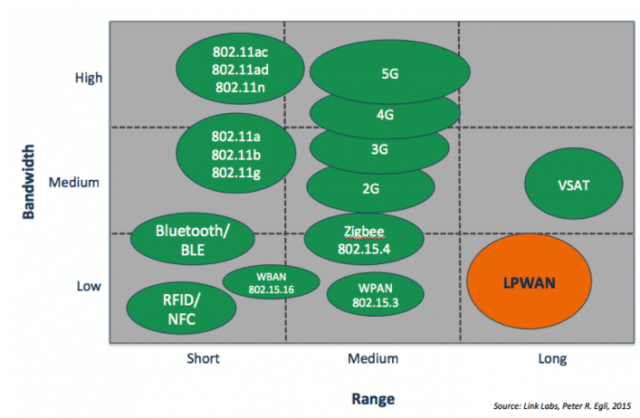
\includegraphics[width=.9\textwidth]{Comparativo-algumas-redes}

    \framebreak

    \textbf{Internet das coisas}: \textit{Internet of things (IoT)}, uma rede que conecta diversas ``coisas'' a internet, através de software, com o objetivo de trocar informações, tais ``coisas'' são dispositivos físicos ou lógicos, podem ser sensores, microcontroladores ou até mesmo objetos que nunca imaginamos tais como geladeiras, televisores, entre outros.

    \framebreak

    \textbf{LoRa}: \textit{Long Range}, é uma tecnologia que atua na camada física para o envio e recebimento de dados. Criado e mantido de forma proprietária pela empresa Semtech, o mesmo utiliza comunicação através de ondas na frequência de radio (\textit{Chirp Spread Spectrum}), para codificar o envio de dados focando em abarcar longas distância a um baixo custo energético.
\end{frame}

\section{Materiais e métodos}
\subsection{Algoritmos utilizados}

\begin{frame}[t,fragile]
    \frametitle{Algoritmo detecção de erros: CRC 16 bits}
\begin{lstlisting}[basicstyle=\small]
uint16_t computeCRC(uint8_t* data_in, uint16_t length) {
    uint8_t bitbang, j;
    uint16_t i, crc_calc = INIT;
    for(i = 0; i < length; i++) {
        crc_calc ^= (((uint16_t)data_in[i]) & 0x00FF);
        for(j = 0; j < 8; j++) {
            bitbang = crc_calc;
            crc_calc >>= 1;
            if(bitbang & 1) crc_calc ^= POLY;
        }
    }
    return (crc_calc & 0xFFFF);
}
\end{lstlisting}
\end{frame}

\begin{frame}
    \frametitle{Controle de fluxo: Stop and Wait}
    \centering
    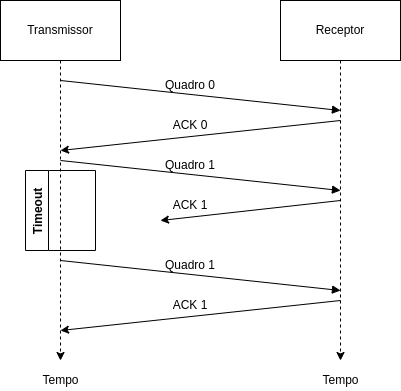
\includegraphics[width=.68\textwidth]{stop_and_wait}
\end{frame}

\subsection{Dispositivos utilizados}
\begin{frame}
    \frametitle{LoRaMESH EndDivice}
    \begin{figure}[!h]
        \centering
        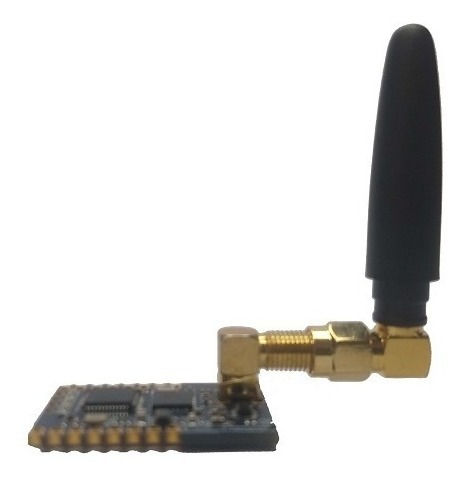
\includegraphics[width=.60\textwidth]{lora}
    \end{figure}
\end{frame}

\begin{frame}
    \frametitle{ESP32}
    \begin{figure}[!h]
        \centering
        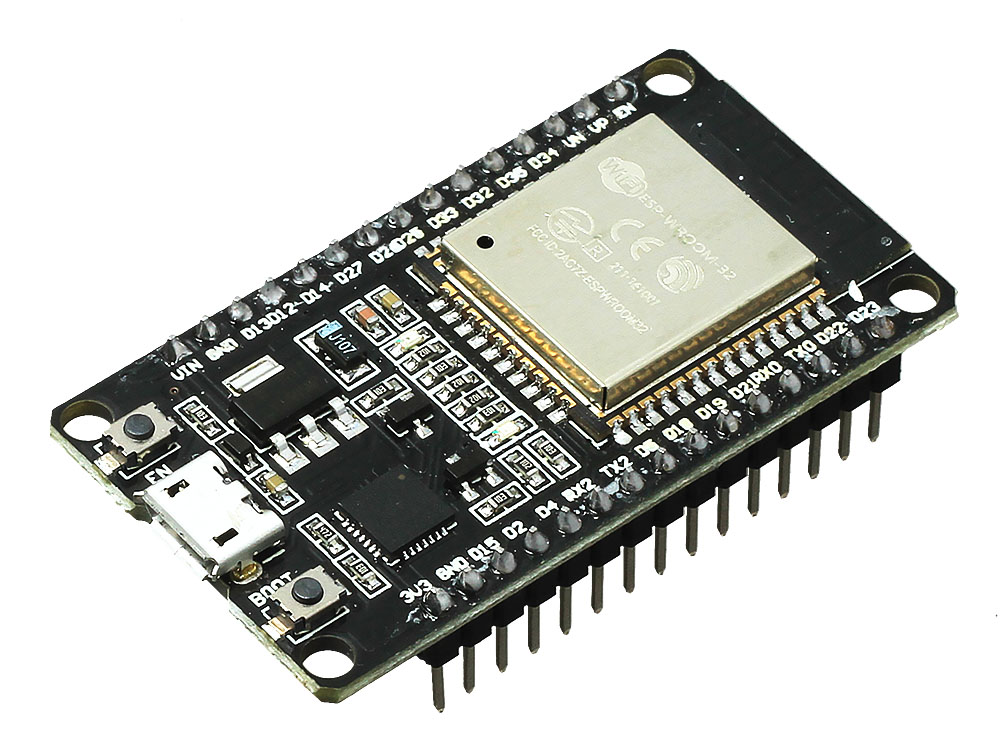
\includegraphics[width=.70\textwidth]{esp}
    \end{figure}
\end{frame}

\begin{frame}
    \frametitle{ESP32-CAM}
    \begin{figure}[!h]
        \centering
        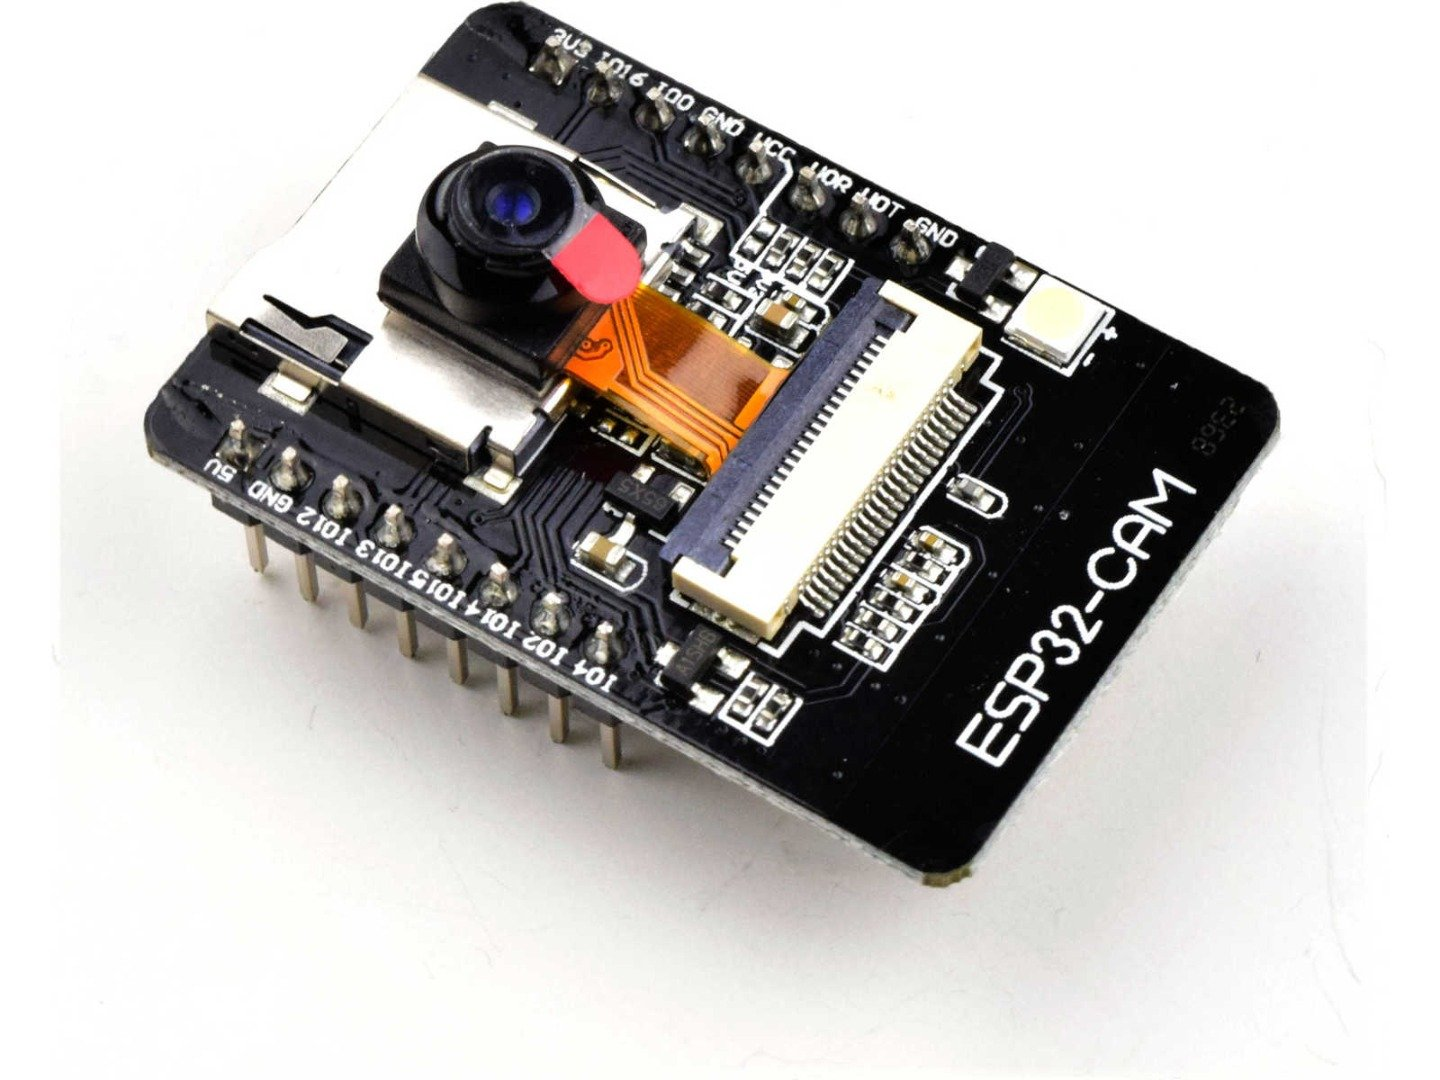
\includegraphics[width=.7\textwidth]{espcam}
    \end{figure}
\end{frame}

\section{Proposta de arquitetura}
\begin{frame}
    \frametitle{Arquitetura}
    \centering
    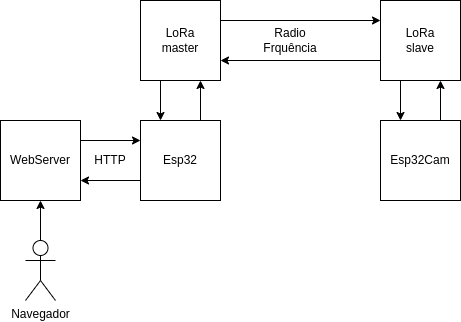
\includegraphics[width=.9\textwidth]{arch}
\end{frame}

\begin{frame}
    \frametitle{End points}
    \begin{itemize}
        \item\textbf{/lora\_img}
            \begin{itemize}
                \item Objetivo: Mostrar no dispositivo do usuário uma imagem JPEG com a última foto salva no dispositivo;
                \item Método: GET;
                \item Retorna: image/jpeg
            \end{itemize}
        \item\textbf{/req\_img/\{\}}
            \begin{itemize}
                \item Objetivo: Fazer com que o LoRa mestre envie uma mensagem pedindo ao dispositivo que tire uma foto e envie;
                \item Parâmetros na url: o id do chip LoRa que vai enviar a imagem;
                \item Método: GET;
                \item Retorna: text/plain, indicando se foi possível ou não fazer a requisição.
            \end{itemize}
    \end{itemize}
\end{frame}

\section{Implementação}
\begin{frame}
    \frametitle{Fluxograma Sender}
    \begin{figure}[!h]
        \centering
        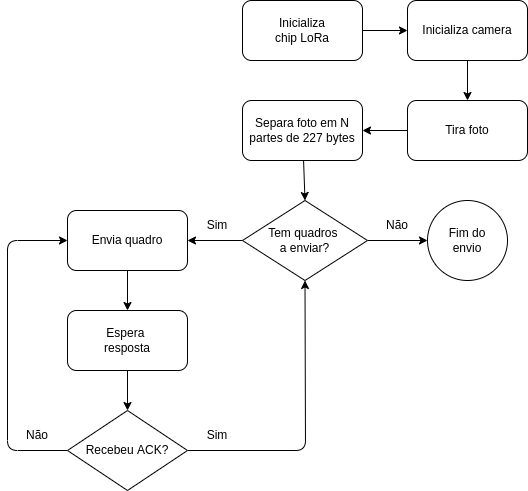
\includegraphics[width=.7\textwidth]{fluxogram_sender}
    \end{figure}
\end{frame}

\begin{frame}
    \frametitle{Fluxograma Receiver}
    \begin{figure}[!h]
        \centering
        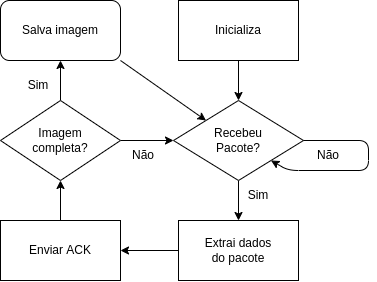
\includegraphics[width=.7\textwidth]{fluxogram_recivier}
    \end{figure}
\end{frame}

\begin{frame}[allowframebreaks]
    \centering
    \frametitle{Estruturas de dados enviadas}
    Para enviar mensagens utilizando o chip LoRa, é preciso seguir o formato:
    \begin{table}[t]
        \begin{tabular}{llll}
            \hline
            \multicolumn{1}{|c|}{ID}      & \multicolumn{1}{c|}{Command} & \multicolumn{1}{c|}{Payload}       & \multicolumn{1}{c|}{CRC}     \\ \hline
            \multicolumn{1}{|c|}{2 bytes} & \multicolumn{1}{c|}{1 byte}  & \multicolumn{1}{c|}{1 - 231 bytes} & \multicolumn{1}{c|}{2 bytes} \\ \hline
                                          &  &  &  \\
                                          &  &  &  \\
                                          &  &  &
        \end{tabular}
    \end{table}

    \framebreak

    \begin{table}[h]
        \centering
        \begin{tabular}{cllll}
            \hline
            \multicolumn{5}{|c|}{Payload}    \\ \hline
            \multicolumn{1}{|c|}{Type}   & \multicolumn{1}{c|}{ID}     & \multicolumn{1}{c|}{Part}   & \multicolumn{1}{c|}{Total}  & \multicolumn{1}{c|}{Message}      \\ \hline
            \multicolumn{1}{|c|}{1 byte} & \multicolumn{1}{c|}{1 byte} & \multicolumn{1}{c|}{1 byte} & \multicolumn{1}{c|}{1 byte} & \multicolumn{1}{c|}{1 - 227 byte} \\ \hline
            \multicolumn{1}{l}{} &  &  &  &  \\
            \multicolumn{1}{l}{} &  &  &  &
        \end{tabular}
    \end{table}

    \begin{itemize}
        \item\textbf{Type}: campo que indica como os próximos bytes devem ser interpretados, podendo ser um ACK, ou uma parte de imagem.
        \item\textbf{ID}: identificador único da imagem;
        \item\textbf{Part}: qual a parte da imagem que está nessa mensagem;
        \item\textbf{Total}: a quantidade total de partes da imagem;
        \item\textbf{Message}: os bytes da imagem
    \end{itemize}
\end{frame}

\begin{frame}[t,fragile]
    \frametitle{Implementação em código}
    \centering
    \begin{lstlisting}[basicstyle=\small]
struct _payload {
    uint8_t byte_array[MAX_PAYLOAD_SIZE];
    uint8_t size;
};

struct _fields {
    uint8_t type, id, part, last_part;
};

union ImagePart {
    _fields fields;
    _payload payload;
};
    \end{lstlisting}
\end{frame}



\section{Resultados}
\begin{frame}
    \frametitle{Teste de Velocidade de transmissão}
    \begin{itemize}
        \item Envia e recebe a resposta em 2 segundos, timeout = 3 segundos;
        \item Máximo descrito na documentação = 21875 bits por segundo.
        \item Máximo utilizando stop and wait = 232 * 8 = 1856 bits por segundo
    \end{itemize}
\end{frame}

\begin{frame}[allowframebreaks]
    \frametitle{Testes no tamanho da imagem}
    Os testes seguiram os seguintes critérios:
    \begin{itemize}
        \item 3 fotos por resolução escolhendo sempre a mediana.
        \item Fotos tiradas do mesmo local na mesma posição;
        \item Imagens em escala de cinsa;
    \end{itemize}
    \framebreak
    \textbf{Compressão constante em 0}
    \begin{table}[!h]
        \centering
        \begin{tabular}{@{}c|c@{}}
            \toprule
            Resolução (pixels) & Tamanho (bytes) \\ \midrule
            640x480            & 73260           \\
            480x320            & 39139           \\
            400x296            & 35916           \\
            320x240            & 23510           \\
            240x176            & 14242           \\
            176x144            & 9147            \\ \bottomrule
        \end{tabular}
        \caption{Mudança de resolução afetando o tamanho da imagem}
        \label{tab:resolution}
    \end{table}
    \framebreak
    \textbf{Resolução constante em 480x320}
    \begin{table}[!h]
        \centering
        \begin{tabular}{@{}c|c@{}}
            \toprule
            Qualidade (0-63) & Tamanho (bytes) \\ \midrule
            0                & 39139           \\
            10               & 8456            \\
            20               & 6371            \\
            30               & 5613            \\
            40               & 5161            \\
            50               & 4842            \\
            60               & 4665            \\
            63               & 4616            \\ \bottomrule
        \end{tabular}
        \caption{Mudança de qualidade da imagem afetando o tamanho}
        \label{tab:quality}
    \end{table}
\end{frame}

\section{Conclusão}
\begin{frame}
    \frametitle{Mão na massa!!}
    \begin{figure}
        \centering
        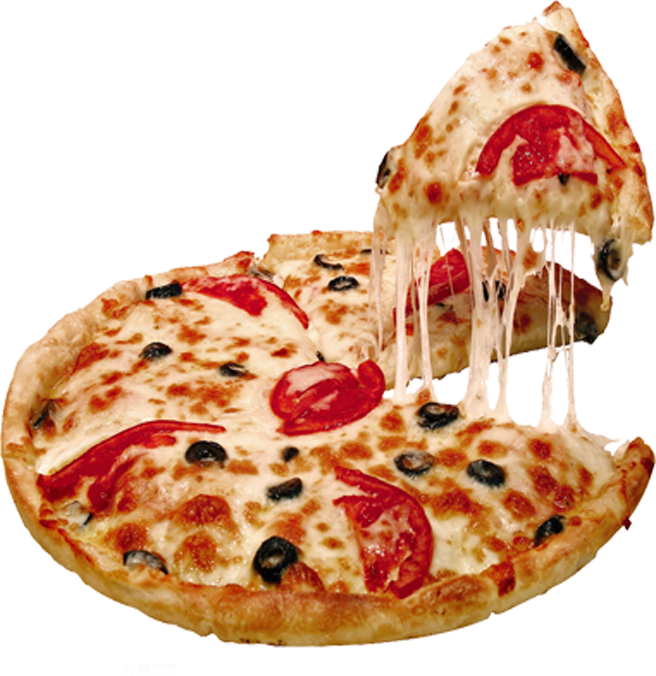
\includegraphics[width=.3\textwidth]{pizza.png}
        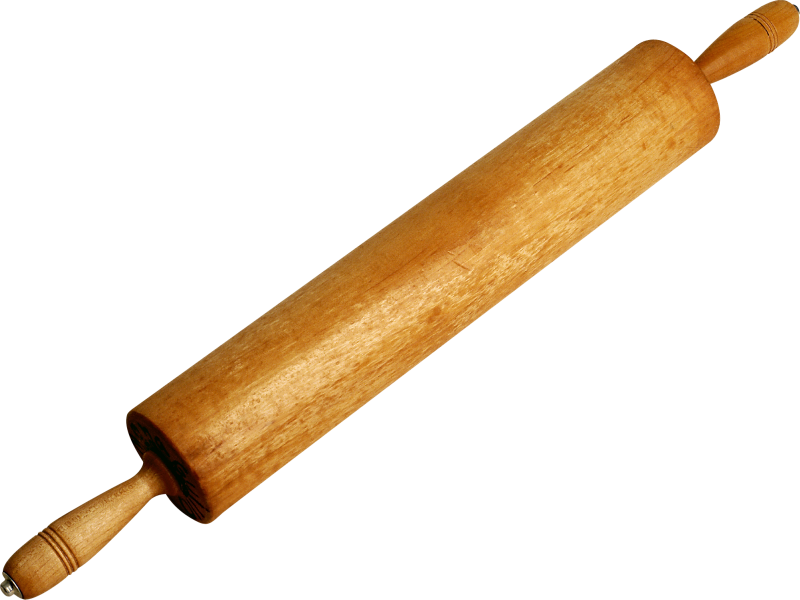
\includegraphics[width=.3\textwidth]{rolo.png}
        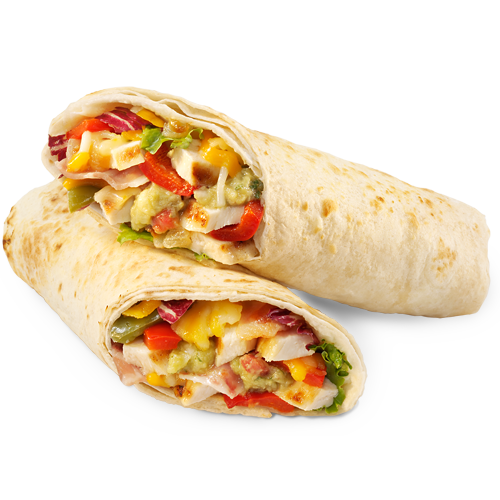
\includegraphics[width=.3\textwidth]{burrito.png}
    \end{figure}
\end{frame}

\begin{frame}
    \frametitle{Agradecimentos}
    \centering
    \Huge{Perguntas?}
    \begin{figure}
        \centering
        
\includegraphics[width=.3\textwidth]{alerta.png}
        
\includegraphics[width=.3\textwidth]{perigo.png}
        
\includegraphics[width=.3\textwidth]{eletricidade.png}
    \end{figure}
    \Huge{Obrigado pela atenção}
\end{frame}

\end{document}
